\documentclass[9pt]{report}
\usepackage{graphicx}
\usepackage[utf8]{inputenc}
%\usepackage[T1]{fontenc}
\usepackage{textcomp}
%\usepackage[dutch]{babel}
\usepackage{amsmath, amssymb}

\begin{document}
\title{Chapter 2 Problems}
\author{Anthony Steel}
\date{\today}
\maketitle
\begin{enumerate}
  \item
    \begin{enumerate}
      \item
      \item
        \textbf{
        Show by explicit construction that two coordinate systems (as opposed
        to the six used in the text) suffice to cover $S^2$ (it is impossible
        to cover $S^2$ with a signle chart, as follows from the fact that $S^2$
        is compact, but every open subset of $\mathbb{R}^2$  is noncompact see
        appendix A.)}
        \begin{figure}
          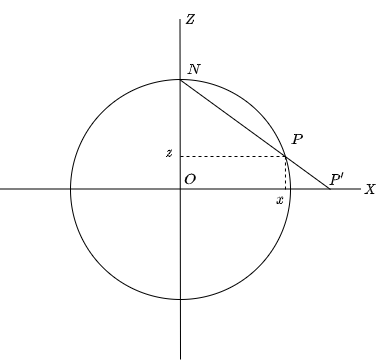
\includegraphics{images/projection.png}
          \caption{Projection of points on a circle into $\mathbb{R}^2$}
          \label{projection}
        \end{figure}

        Consider the collection of two subsets, $O_N$ and $O_S$. $O_N$ contains
        all the points in the set $S^2$ except the north pole $(0, 0, 1)$, and $O_S$ contains
        all the points in $S^$ except the south pole $(0, 0, -1)$. Together
        this collection contains every point in $S^2$ thereby satisfying property
        $1$ required for a manifold.


        Next we must determine two maps, $\psi_N$ and $\psi_S$ for $O_N$ and
        $O_S$ respectively, and show that they are one-to-one and map $S^2$ to
        $\mathbb{R}^2$. To construct these maps consider Figure \ref{projection}.
        Pictured are all the points in $S^2$ which lie in the $X$-$Z$ plane.
        We will use this diagram to construct the map $\psi_$.

        Draw a line from the north pole $N$ that intersects the $S^2$ at a point
        $P$ and the $X$ axis at $P^\prime$. The point $P$ has coordinates
        $(x,0,z)$. The triangles $NzP$ and $NOP^\prime$ can be related using
        similar triangles. This will give a relation between the point $P$
        and $P^\prime$.
        \[
        \begin{align}
          \frac{OP^\prime}{NO}&= \frac{zP}{Nz} \\
          P^\prime &= \frac{x}{1-z}\\
        \end{align}
      \]
      $P^\prime$ is equivalent to mapping the any point $P$ into the $X-Y$ plane
      and we will denote this coordinate in the $X$ direction $X^\prime$. The same
      argument can be made to find $Y^\prime$ by replacing $x$ in the above
      equation with $y$. Therefore:
      \[
        O^N : S^2 \rightarrow \mathbb{R}^2 = {(X^\prime, Y^\prime) = (\frac{x}{1-z}, \frac{y}{1-z})}
      \]
        $\psi_N$ can be constructed in a similar manner but replacing $z$ with
        $-z$:
        \[
          (X^\prime, Y^\prime) = (\frac{x}{1+z}, \frac{y}{1+z})
        \]
      Each of these maps are clearly one to one and onto.
      \[
        (X, Y) = (\frac{x}{1-z}, \frac{y}{1-z})
      \]
      \[
        (x, y, z) = (\frac{2X}{1+X^2+Y^2}. \frac{2Y}{1+X^2+Y^2}, \frac{-1+X^2+Y^2}{1+X^2+Y^2})
      \]
      $\psi_N : O_N \rightarrow U_N\subset \mathbb{R}^2$ and
      $\psi_S : O_S \rightarrow U_S\subset \mathbb{R}^2$. In order to satisfy
      property 3 of manifolds we must show that $\psi_N \circ \psi_S^{-1}$
      and $\psi_S \circ \psi_N^{-1}$ the subsets of the map are open and the maps
      are infinitely differentiable.
      \[
        (X^\prime, Y^\prime) = (\frac{2X}{(1+X^2+Y^2)(1-\frac{-1+X^2+Y^2}{1+X^2+Y^2})},
                  \frac{2Y}{(1+X^2+Y^2)(1-\frac{-1+X^2+Y^2}{1+X^2+Y^2})})
      \]
      \[
        (X^\prime, Y^\prime) = (\frac{2X}{1+X^2+Y^2+1-X^2-Y^2},
                  \frac{2Y}{1+X^2+Y^2+1-X^2-Y^2}) = (X, Y)
      \]
    \end{enumerate}
  \item
    \textbf{Prove that any smooth function $F:\mathbb{R}^n \rightarrow \mathbb{R}$
    can be written in the form equation (2.2.2)}
  \item
    \begin{enumerate}
    \item
    \textbf{Verify that the commutator, defined by equation (2.2.14),
    satisfies the linearity and Leibnitz properties, and hence defines a
    vector field}
  \[
    \begin{align}
    [v,w](f+g) &= v(w(f+g)) - w(v(f+g))\\
               &= v(w(f)+w(g))-w(v(f)+v(g))\\
               &= v(w(f))+v(w(g))-w(v(f))-w(v(g))\\
               &= v(w(f))-w(v(f))+v(w(g))-w(v(g))\\
               &= [v,w]f+[v,w]g\\
    \end{align}
  \]
  Therefore the commutator satisfies the linearity property in $v$. The same
  procedure can be applied symmetrically to $w$.
  \[
    \begin{align}
      [v,w](fg) &= v(w(fg)) - w(v(fg))\\
                &= v(w(f)g+fw(g)) - w(v(f)g+fv(g))\\
                &= v(w(f)g)+v(fw(g)) - w(v(f)g)-w(fv(g))\\
                &= v(w(f))g+w(f)v(g)+v(f)w(g)+fv(w(g))\\
                &-w(v(f))g-v(f)w(g)-w(f)v(g)-fw(v(g))\\
                &= v(w(f))g+f(v(w(g))-w(v(f))g-fw(v(g))\\
                &= f(v(w(g))-fw(v(g))+v(w(f))g-w(v(f))g\\
                &= f\Big((v(w(g))-w(v(g))\Big)+g\Big(v(w(f))-w(v(f))\Big)\\
                &= f[v,w](g)+g[v,w](f)
    \end{align}
  \]
  \item \textbf{Let $X$, $Y$, $Z$ be smooth vector fields on a manifold $M$. Verify
    that their commutator satisfies the Jacobi identity:}
  \[
    [[X,Y],Z] + [[Y,Z],X] + [[Z,X],Y] = 0
  \]
  Expand $[[X,Y],Z]$:
  \[
    \begin{align}
      [[X,Y],Z](f) &= [X,Y]Z(f)-Z[X,Y](f)\\
                   &= X(Y(Z(f)))-Y(X(Z(f)))-Z(X(Y(f))-Y(Z(f))) \\
                   &= X(Y(Z(f)))-Y(X(Z(f)))-Z(X(Y(f)))+Z(Y(Z(f))) \\
                   &= X(Y(Z(f)))-Y(X(Z(f)))-Z(X(Y(f)))+Z(Y(Z(f))) \\
    \end{align}
  \]
  Now cyclically permute $X$,$Y$,$Z$:
  \[
    \begin{align}
                   &= \underbrace{X(Y(Z(f)))}_a-\underbrace{Y(X(Z(f)))}_{-g}-\underbrace{Z(X(Y(f)))}_{-e}+\underbrace{Z(Y(X(f)))}_b \\
                   &+ \underbrace{Y(Z(X(f)))}_c-\underbrace{Z(Y(X(f)))}_{-b}-\underbrace{X(Y(Z(f)))}_{-a}+\underbrace{X(Z(Y(f)))}_d \\
                   &+ \underbrace{Z(X(Y(f)))}_e-\underbrace{X(Z(Y(f)))}_{-d}-\underbrace{Y(Z(X(f)))}_{-c}+\underbrace{Y(X(Z(f)))}_g \\
                   &= 0
    \end{align}
  \]
\item \textbf{Let $Y_1,\ldots,Y_n$ be smooth vector fields on an n-dimensional
  $M$ such that at each $p\in M$ they form a basis of the tangent space $V_p$.
Then, at each point, we may expand each commutator $[Y_\alpha, Y_\beta]$ in
this basis, thereby defining the functions $C^\gamma_\alpha_\beta=-C^\gamma_\beta_\alpha$ by}
\[
  [Y_\alpha, Y_\beta] = \sum_\gamma C^\gamma_\alpha_\beta Y_\gamma
\]
  \textbf{Use the Jacobi identity to derive an equation satisfied by $C^\gamma_\alpha_\beta$.}\\\\
  Consider:
  \[
    \begin{align*}
      [[Y_\alpha, Y_\beta], Y_\sigma] &= [C^\gamma_\alpha_\beta Y_\gamma,Y_\sigma]\\
    &= C^\gamma_\alpha_\beta Y_\gamma Y_\sigma - Y_\sigma C^\gamma_\alpha_\beta Y_\gamma \\
    &= C^\gamma_\alpha_\beta Y_\gamma Y_\sigma - C^\gamma_\alpha_\beta Y_\sigma Y_\gamma \\
    &= C^\gamma_\alpha_\beta [Y_\gamma Y_\sigma - Y_\sigma Y_\gamma] \\
    &= C^\gamma_\alpha_\beta \Big(Y_\gamma Y_\sigma - Y_\sigma Y_\gamma\Big) \\
    &= C^\gamma_\alpha_\beta [Y_\gamma, Y_\sigma] \\
    &= C^\gamma_\alpha_\beta C^\epsilon_\gamma_\sigma Y_\epsilon \\
    \end{align*}
  \]
  Therefore the Jacobi identity gives:
  \[
  \begin{align*}
    [[Y_\alpha, Y_\beta],Y_\sigma]+[[Y_\beta, Y_\sigma],Y_\alpha]+[[Y_\sigma, Y_\alpha],Y_\beta] &= 0 \\
    C^\gamma_\alpha_\beta C^\epsilon_\gamma_\sigma Y_\epsilon
    + C^\gamma_\beta_\sigma C^\epsilon_\gamma_\alpha Y_\epsilon + C^\gamma_\sigma_\alpha C^\epsilon_\gamma_\beta Y_\epsilon &=0 \\
    (C^\gamma_\alpha_\beta C^\epsilon_\gamma_\sigma+ C^\gamma_\beta_\sigma C^\epsilon_\gamma_\alpha + C^\gamma_\sigma_\alpha C^\epsilon_\gamma_\beta) Y_\epsilon &=0 \\
    \end{align*}
  \]
  Therefore the equations satisfied by the functions are:
  \[
    (C^\gamma_\alpha_\beta C^\epsilon_\gamma_\sigma+ C^\gamma_\beta_\sigma C^\epsilon_\gamma_\alpha + C^\gamma_\sigma_\alpha C^\epsilon_\gamma_\beta) =0
  \]
  \end{enumerate}
  \item
  \begin{enumerate}
    \item \textbf{Show that in any coordinate basis, the components of the
      commutator of two vector fields $v$ and $w$ are given by}
      \[
        [v,w]^\mu = \sum_\nu \Big( v^\nu \frac{\partial w^\mu}{\partial x^\nu}
        - w^\nu\frac{\partial v^\mu}{\partial x^\nu} \Big)
      \]

      \[
  \begin{align}
    [v,w](f) &= v(w(f)) - w(v(f)) \\
   &= v(w^\mu\frac{\partial f}{\partial x^\mu})-w(v^\mu \frac{\partial f}{\partial x^\mu} )\\
   &= v^\nu \frac{\partial}{\partial x^\nu} (w^\mu\frac{\partial f}{\partial x^\mu})-
      w^\nu \frac{\partial}{\partial x^\nu} (v^\mu \frac{\partial f}{\partial x^\mu} )\\
   &= v^\nu \Big( \frac{\partial w^\mu}{\partial x^\nu}\frac{\partial f}{\partial x^\mu}
     + w^\mu \frac{\partial f}{\partial x^\nu x^\mu}\Big)-
     w^\nu \Big( \frac{\partial v^\mu}{\partial x^\nu}\frac{\partial f}{\partial x^\mu}
     + v^\mu \frac{\partial f}{\partial x^\nu x^\mu}\Big)\\
   &= v^\nu \frac{\partial w^\mu}{\partial x^\nu}\frac{\partial f}{\partial x^\mu}
     + v^\nu w^\mu \frac{\partial f}{\partial x^\nu x^\mu}
   - w^\nu \frac{\partial v^\mu}{\partial x^\nu}\frac{\partial f}{\partial x^\mu}
   - w^\nu v^\mu \frac{\partial f}{\partial x^\nu x^\mu}\\
   &= v^\nu \frac{\partial w^\mu}{\partial x^\nu}\frac{\partial f}{\partial x^\mu}
   - w^\nu \frac{\partial v^\mu}{\partial x^\nu}\frac{\partial f}{\partial x^\mu}
   + \Big(v^\nu w^\mu \frac{\partial f}{\partial x^\nu x^\mu}
   - w^\nu v^\mu \frac{\partial f}{\partial x^\nu x^\mu}\Big)\\
  \end{align}
      \]
  Using the equality of mixed partial derivatives we can relabel the indices:
  \[
  \begin{align}
   &= v^\nu \frac{\partial w^\mu}{\partial x^\nu}\frac{\partial f}{\partial x^\mu}
   - w^\nu \frac{\partial v^\mu}{\partial x^\nu}\frac{\partial f}{\partial x^\mu}
   + \Big(v^\nu w^\mu \frac{\partial f}{\partial x^\nu x^\mu}
   - w^\mu v^\nu \frac{\partial f}{\partial x^\mu x^\nu}\Big)\\
   &= v^\nu \frac{\partial w^\mu}{\partial x^\nu}\frac{\partial f}{\partial x^\mu}
   - w^\nu \frac{\partial v^\mu}{\partial x^\nu}\frac{\partial f}{\partial x^\mu}\\
   &= \Big(v^\nu \frac{\partial w^\mu}{\partial x^\nu}
   - w^\nu \frac{\partial v^\mu}{\partial x^\nu}\Big) \frac{\partial f}{\partial x^\mu}\\
   &= [v,w]^\mu\frac{\partial f}{\partial x^\mu}\\
  \end{align}
  \]
  \item
    \textbf{Let $Y_1$, $\ldots$, $Y_n$ be as in problem 3(c). Let $Y^{1^*}$,$\ldots$,
    $Y^{n^*}$ be the dual basis. Show that the components $(Y^{\gamma^*})_\mu$
     of $Y^{\gamma^*}$ in any coordinate basis satisfy}
     \[
     \frac{\partial (Y^{\gamma^*})_\mu}{\partial x^\nu} - \frac{\partial (Y^{\gamma^*})_\nu}{\partial x^\mu}
     = \sum_{\alpha, \beta} C^\gamma_\alpha_\beta(Y^{\alpha^*})_\mu (Y^{\beta^*})_\nu
     \]
    Considering the commutator used in problem 3(c):
  \[
    [Y_\alpha, Y_\beta] = \sum_\gamma C^\gamma_\alpha_\beta Y_\gamma
  \]
  Act the commutator on a dual vector $Y^{\gamma^*}$:
  \[
    [Y_\alpha, Y_\beta]Y^{\gamma^*}= \sum_\gamma C^\gamma_\alpha_\beta Y_\gamma Y^{\gamma^*}
  \]

  Start with the right hand side.
  \end{enumerate}
  \item
  \item
  \item
  \item
  \begin{enumerate}

  \item \textbf{The metric of flat, three-dimensional Euclidean space is:} \[
      ds^2 = dx^2 + dy^2 + dz^2
  \]
  \textbf{Show that the metric components $g_{uv}$ in spherical polar
  coordinates $r, \theta, \phi$ defined by:}
  \[
    \begin{align*}
      &r = \sqrt{x^2 + y^2 + z^2} \\
      &\cos\theta = \frac{z}{r}, \\
      &\tan\phi = \frac{y}{x}
    \end{align*}
  \]
  \textbf{is given by:}
  \[
    s^2 = dr^2 + r^2 d\theta^2 + r^2 \sin^2\thetad\phi^2
  \]
 $g_{uv}$ is a tensor of type $\left( 0,2 \right) $ and therefore transforms as:
  \[
    g_{\mu',\nu'} = g_{\mu,\nu} \frac{\partial x^\mu}{\partial x^{\mu'}}\frac{\partial x^\nu}{\partial x^{\nu'}}
  \]
  (see page 22 for the general \textit{tensor transformation law}). The above
  equation uses Einstein index notation indicating that $\mu$ and $\nu$ are to
  to be summed from 1 to 3 and the free indices, $\mu'$ and $\nu'$, are
  enumerated through all possible combinations. Therefore the components that
  need to be calculated are:
  \[
    \begin{matrix}
      g_{r,r}  && g_{r,\theta} && g_{r,\phi} \\
      g_{\theta, r} && g_{\theta,\theta} && g_{\theta,\phi} \\
      g_{\phi,r} && g_{\phi,\theta} && g_{\phi,\phi}
    \end{matrix}
  \]
  Starting with:
  \[
    g_{\mu',\nu'} =
    \sum_{\mu=1}^{3} \sum_{\nu=1}^{3} g_{\mu,\nu} \frac{\partial x^\mu}{\partial x^{\mu'}} \frac{\partial x^\nu}{\partial x^{\nu'}}
  \]
  \[
    = \sum_{\mu=1}^{3}
    g_{\mu, 1} \frac{\partial x^\mu}{\partial x^{\mu'}} \frac{\partial x^1}{\partial x^{\nu'}} +
    g_{\mu, 2} \frac{\partial x^\mu}{\partial x^{\mu'}} \frac{\partial x^2}{\partial x^{\nu'}} +
    g_{\mu, 3} \frac{\partial x^\mu}{\partial x^{\mu'}} \frac{\partial x^3}{\partial x^{\nu'}}
  \]
  \[
    \begin{align*}
    =&\
     g_{1,1}\frac{\partial x^1}{\partial x^{\mu'}}\frac{\partial x^1}{\partial x^{\nu'}}
    +g_{1,2}\frac{\partial x^1}{\partial x^{\mu'}}\frac{\partial x^2}{\partial x^{\nu'}}
    +g_{1,3}\frac{\partial x^1}{\partial x^{\mu'}}\frac{\partial x^3}{\partial x^{\nu'}}\\
    &\ g_{2,1}\frac{\partial x^2}{\partial x^{\mu'}}\frac{\partial x^1}{\partial x^{\nu'}}
    +g_{2,2}\frac{\partial x^2}{\partial x^{\mu'}}\frac{\partial x^2}{\partial x^{\nu'}}
    +g_{2,3}\frac{\partial x^2}{\partial x^{\mu'}}\frac{\partial x^3}{\partial x^{\nu'}}\\
    &\
     g_{3,1}\frac{\partial x^2}{\partial x^{\mu'}}\frac{\partial x^1}{\partial x^{\nu'}}
    +g_{3,2}\frac{\partial x^2}{\partial x^{\mu'}}\frac{\partial x^2}{\partial x^{\nu'}}
    +g_{3,3}\frac{\partial x^2}{\partial x^{\mu'}}\frac{\partial x^3}{\partial x^{\nu'}}\\
    \end{align*}
  \]
  Substituting the notation for the indices in flat, orthonormal Euclidean
  space:
  \[
    \begin{align*}
    =&\
     g_{x,x}\frac{\partial x}{\partial x^{\mu'}}\frac{\partial x}{\partial x^{\nu'}}
    +g_{x,y}\frac{\partial x}{\partial x^{\mu'}}\frac{\partial y}{\partial x^{\nu'}}
    +g_{x,z}\frac{\partial x}{\partial x^{\mu'}}\frac{\partial z}{\partial x^{\nu'}}\\
    &\ g_{y,x}\frac{\partial y}{\partial x^{\mu'}}\frac{\partial x}{\partial x^{\nu'}}
    +g_{y,y}\frac{\partial y}{\partial x^{\mu'}}\frac{\partial y}{\partial x^{\nu'}}
    +g_{y,z}\frac{\partial y}{\partial x^{\mu'}}\frac{\partial z}{\partial x^{\nu'}}\\
    &\
     g_{z,x}\frac{\partial y}{\partial x^{\mu'}}\frac{\partial x}{\partial x^{\nu'}}
    +g_{z,y}\frac{\partial y}{\partial x^{\mu'}}\frac{\partial y}{\partial x^{\nu'}}
    +g_{z,z}\frac{\partial y}{\partial x^{\mu'}}\frac{\partial z}{\partial x^{\nu'}}\\
    \end{align*}
  \]
  The off diagonal elements of the Euclidean metric are zero:
  \[
    g_{x,y} = g_{y,x} = g_{x,z} = g_{z,x} = g_{y,z} = g_{z,y} = 0
  \]
  and the diagonal components are one:
  \[
    g_{x,x} = g_{y,y} = g_{z,z} = 1
  \]
  This reduces the above summation from nine expressions to the following three: \[
    g_{\mu',\nu'} =
    \frac{\partial x}{\partial x^{\mu'}} \frac{\partial x}{\partial x^{\nu'}} +
    \frac{\partial y}{\partial x^{\mu'}} \frac{\partial y}{\partial x^{\nu'}} +
    \frac{\partial z}{\partial x^{\mu'}} \frac{\partial z}{\partial x^{\nu'}}
  \]
  For indices where $\mu'=\nu'$
  \[
    g_{\mu', \mu'} =
    \Bigg( \frac{\partial x}{\partial x^{\mu'}}\Bigg)^2+
    \Bigg(\frac{\partial y}{\partial x^{\mu'}}\Bigg)^2+
    \Bigg(\frac{\partial z}{\partial x^{\mu'}}\Bigg)^2
  \]
  Therefore the six unique components that need to be calculated to find the
  components of the metric in spherical polar coorindates are:
  \[
    \begin{align*}
    g_{r,r} &=
    \Bigg( \frac{\partial x}{\partial r}\Bigg)^2+
    \Bigg(\frac{\partial y}{\partial r}\Bigg)^2+
    \Bigg(\frac{\partial z}{\partial r}\Bigg)^2\\
    g_{r,\theta} &= g_{\theta,r} = \frac{\partial x}{\partial r} \frac{\partial x}{\partial \theta}
    +\frac{\partial y}{\partial r} \frac{\partial y}{\partial \theta}
    +\frac{\partial z}{\partial r} \frac{\partial z}{\partial \theta}\\
    g_{r,\phi} &= g_{\phi,r} = \frac{\partial x}{\partial r} \frac{\partial x}{\partial \phi}
    + \frac{\partial y}{\partial r} \frac{\partial y}{\partial \phi}
    + \frac{\partial z}{\partial r} \frac{\partial z}{\partial \phi}\\
    g_{\theta,\theta} &=
    \Bigg( \frac{\partial x}{\partial \theta}\Bigg)^2+
    \Bigg(\frac{\partial y}{\partial \theta}\Bigg)^2+
    \Bigg(\frac{\partial z}{\partial \theta}\Bigg)^2\\
    g_{\theta,\phi} &= g_{\phi,\theta} = \frac{\partial x}{\partial \theta} \frac{\partial x}{\partial \phi}
    +\frac{\partial y}{\partial \theta} \frac{\partial y}{\partial \phi}
    +\frac{\partial z}{\partial \theta} \frac{\partial z}{\partial \phi} \\
    g_{\phi,\phi} &=
    \Bigg( \frac{\partial x}{\partial \phi}\Bigg)^2+
    \Bigg(\frac{\partial y}{\partial \phi}\Bigg)^2+
    \Bigg(\frac{\partial z}{\partial \phi}\Bigg)^2
    \end{align*}
  \]
  To take the above derivatives, find an equation for $x$, $y$, $z$ in terms of $r$, $\theta$, $\phi$.
  Starting by finding $x$:
  \[
    \begin{align*}
      &r = \sqrt{x^2 + y^2 + z^2} \to r^2= x^2+z^2+y^2,\\
      &\cos\theta = \frac{z}{r} \to z = r\cos\theta, \\
      &\tan\phi = \frac{y}{x} \to y = x\tan\phi
    \end{align*}
  \]
  Substituting the second and third equation into the first gives:
  \[
    \begin{align*}
      r^2&=x^2+(r\cos\theta)^2+(x\tan\phi)^2\\
      r^2&=x^2+r^2\cos^2\theta+x^2\tan^2\phi\\
      r^2-r^2\cos\theta&=x^2+x^2\tan^2\phi\\
      (1-\cos^2\theta)r^2&=(1+\tan^2\phi)x^2\\
      r^2\sin^2\theta &=(1+\tan^2\phi)x^2\\
      x&=r\frac{\sin\theta}{\sqrt{1+\tan^2\phi}}\\
    \end{align*}
  \]
  Therefore the equations for $x$, $y$, $z$ in terms of $r$, $\theta$, $\phi$:
  \[
    x = r \frac{\sin\theta}{\sqrt{1+\tan^2\phi} }\text{,\ \ }
    y = r \tan\phi \frac{\sin \theta}{\sqrt{1+\tan^2\phi}}\text{,\ \ }
    z = r \cos\theta
  \]
  Find all the necessary derivatives:
  \[
    \begin{align*}
    \frac{\partial x}{\partial r} &= \frac{\sin\theta}{\sqrt{1+\tan^2\phi}}\\
    \frac{\partial x}{\partial \theta} &= -r\frac{\cos\theta}{\sqrt{1+\tan^2\phi}}\\
    \frac{\partial x}{\partial \phi} &= -r \sin \theta \frac{\tan\phi \sec^2\phi}{(1+\tan^2\phi)^\frac{3}{2}} \\
    \frac{\partial y}{\partial r} &= \tan\phi\frac{\sin\theta}{\sqrt{1+\tan^2\phi} }\\
    \frac{\partial y}{\partial \theta} &= -r \tan\phi\frac{\cos\theta}{\sqrt{1+\tan^2\phi}}\\
    \frac{\partial y}{\partial \phi} &= -r\sin\theta \frac{\sec^2\phi}{(1+\tan^2\phi)^\frac{3}{2}}\\
    \frac{\partial z}{\partial r} &= \cos\theta\\
    \frac{\partial z}{\partial \theta} &= r\sin\theta\\
    \frac{\partial z}{\partial \phi} &= 0
    \end{align*}
  \]
  Then compute the components of the metric in spherical polar coordinates:
  \[
    \begin{align*}
      g_{r,r}&=\frac{\sin\theta^2}{1+\tan^2\phi} + \frac{\sin^2\theta}{1+\tan^2\phi}\tan^2\phi + \cos^2\theta\\
      &=\frac{\sin\theta^2 + \sin^2\theta\tan^2\phi}{1+\tan^2\phi} +\frac{(1+\tan^2\phi)\cos^2\theta}{1+\tan^2\phi}\\
      &=\frac{\sin\theta^2 + \sin^2\theta\tan^2\phi+(1+\tan^2\phi)\cos^2\theta}{1+\tan^2\phi}\\
      &=\frac{\sin^2\theta + \cos^2\theta+\sin^2\theta\tan^2\phi+\tan^2\phi\cos^2\theta}{1+\tan^2\phi}\\
      &=\frac{1+\tan^2\phi}{1+\tan^2\phi}\\
      &=1\\
    \end{align*}
  \]
  \[
    \begin{align*}
      g_{\theta,\theta}&=
      r^2 \frac{\cos^2\theta}{1+\tan^2\phi}+
      r^2 \frac{\cos^2\theta}{1+\tan^2\phi}\tan^2\phi
      + r^2\sin^2\theta\\
      &= r^2 \frac{\cos^2\theta}{1+\tan^2\phi}+
      r^2 \frac{\cos^2\theta}{1+\tan^2\phi}\tan^2\phi
      + r^2\sin^2\theta\frac{1+\tan^2\phi}{1+\tan^2\phi}\\
      &=r^2 \frac{\cos^2\theta+\cos^2\theta\tan^2\phi+\sin^2\theta+\tan^2\phi\sin^2\theta}{1+\tan^2\phi}\\
      &=r^2 \frac{(\cos^2\theta+\sin^2\theta)+(\cos^2\theta+\sin^2\theta)\tan^2\phi}{1+\tan^2\phi}\\
      &=r^2 \frac{1+\tan^2\phi}{1+\tan^2\phi}\\
      &=r^2 \\
    \end{align*}
  \]
  \[
    \begin{align*}
      g_{\phi,\phi}&= r^2\sin^2\theta\Bigg(\frac{1}{(1+\tan^2\phi)^{3}\cos^4\phi} +
      \frac{\sin^2\phi}{(1+\tan^2\phi)^3\cos^6x}\Bigg)\\
      &=r^2\sin^2\theta\Bigg(\frac{\cos^2\phi+\sin^2\phi}{(1+\tan^2\phi)^3\cos^6\phi}\Bigg)\\
      &=r^2\sin^2\theta\frac{1}{\big(\frac{\sin^2\phi+\cos^2\phi}{\cos^2\phi}\big)^3\cos^6\phi}\\
      &=r^2\sin^2\theta
    \end{align*}
  \]
  \[
    \begin{align*}
      g_{\theta, r} = g_{r,\theta} &=
    g_{x,x} \frac{\partial x}{\partial r} \frac{\partial x}{\partial \theta}
    + g_{y,y} \frac{\partial y}{\partial r} \frac{\partial y}{\partial \theta}
    + g_{z,z} \frac{\partial z}{\partial r} \frac{\partial z}{\partial \theta}\\
    &= -r\frac{\sin\theta\cos\theta}{1+\tan^2\phi}-r\frac{\sin\theta\cos\theta}{1+\tan^2\phi}\tan^2\phi
    + r\sin\theta\cos\theta\\
    &= -r \frac{\sin\theta \cos\theta}{1+\tan^2\phi}(1+\tan^2\phi) + r \sin\theta \cos\theta \\
    &= - r \sin\theta \cos\theta + r \sin\theta \cos\theta \\
    &= 0
    \end{align*}
  \]
  \[
  \[
    \begin{align*}
      g_{r,\phi} = g_{\phi,r} &=
    g_{x,x} \frac{\partial x}{\partial r}  \frac{\partial x}{\partial \phi} +
    g_{y,y} \frac{\partial y}{\partial r} \frac{\partial y}{\partial \phi} +
    g_{z,z} \frac{\partial z}{\partial r} \frac{\partial z}{\partial \phi} \\
    &=
     -r \sin\theta \cos\theta \frac{\tan\phi \sec^2\phi}{(1+\tan^2\phi)^2}
    + r \cos\theta\sin\theta \frac{\tan\phi \sec^2\phi}{(1+\tan^2\phi)^2}\\
    &= 0
    \end{align*}
  \]
  \[
    \begin{align*}
      g_{\theta,\phi} = g_{\phi, \theta} &=
    g_{x,x}\frac{\partial x}{\partial \theta} \frac{\partial x}{\partial \phi}+
    g_{y,y}\frac{\partial y}{\partial \theta} \frac{\partial y}{\partial \phi}+
    g_{z,z}\frac{\partial z}{\partial \theta} \frac{\partial z}{\partial \phi}\\
    &=-r\frac{\cos\theta}{\sqrt{1+\tan^2\phi}}\Bigg(-r\sin\theta\frac{\tan\phi\sec^2\phi}{(1+\tan^2\phi)^\frac{3}{2}}\Bigg)
    -r\tan\phi\frac{\cos\theta}{\sqrt{1+\tan^2\phi}}\Bigg(r \sin\theta \frac{\sec^2\phi}{(1+\tan^2\phi)^\frac{3}{2}} \Bigg)\\
  &=r^2\sin\theta\cos\theta\frac{\tan\phi\sec^2\phi}{(1+\tan^2\phi)^2}
  -r^2 \sin \theta \cos\theta\frac{\tan\phi\sec^2\phi}{(1+\tan^2\phi)^2}\\
  &= 0
    \end{align*}
  \]
  Therefore the metric components in spherical polar coordinates are:
  \[
    g_{\mu, \nu} =
    \begin{bmatrix}
      1 && 0 && 0 \\
      0 && r^2 && 0 \\
      0 && 0 && r^2\sin^2\theta
    \end{bmatrix}
  \]
  \item
  \textbf{The spacetime metric of special relativity is}
  \[
  ds^2=-dt^2+dx^2+dy^2+dz^2
  \]
  \textbf{Find the components, $g_{\mu\nu}$ and $g^{\mu\nu}$, of the metric and
  inverse metric in "rotating coordinates", defined by}
  \[
    \begin{align*}
      t'&=t\\
      x'&=(x^2+y^2)^\frac{1}{2}\cos(\phi-wt)\\
      y'&=(x^2+y^2)^\frac{1}{2}\sin(\phi-wt)\\
      z'&=z
    \end{align*}
  \]
  \textbf{where $\tan\phi = \frac{y}{x}$}\\
  It is easier differentiate with respect to the primed coordinates so find
  $g^{\mu\nu}$ first. First writting the primed coordinates in terms of the
  unprimed:
  \[
  \begin{align*}
    t' &= t\\
    x' &= (x^2+y^2)^\frac{1}{2}\cos(\tan^{-1}\frac{y}{x} - wt)\\
    y' &= (x^2+y^2)^\frac{1}{2}\sin(\tan^{-1} \frac{y}{x} - wt)\\
    z' &= z
  \end{align*}
  \]
  Find all the necessary derivatives:
  \[
    \begin{align*}
    \frac{\partial t'}{\partial t} &= 1\\
    \frac{\partial t'}{\partial x} &= \frac{\partial t'}{\partial y} =
    \frac{\partial t}{\partial z} = 0\\
    \\
    \frac{\partial x'}{\partial t} &= -w\sqrt{x^2+y^2} \sin(\tan^{-1}\frac{y}{x}-wt)\\
    \frac{\partial x'}{\partial x} &=
    \frac{x\cos(\tan^{-1} \frac{y}{x}-\omega t)+y\sin(\tan^{-1}\frac{y}{x}-\omega t)}{\sqrt{x^2+y^2}}\\
    \frac{\partial x'}{\partial y} &=
    \frac{-x\sin(\tan^{-1} \frac{y}{x}-\omega t)+y\cos(\tan^{-1}\frac{y}{x}-\omega t)}{\sqrt{x^2+y^2}}\\
    \frac{\partial x'}{\partial z} &= 0\\
    \\
    \frac{\partial y'}{\partial t} &= -w\sqrt{x^2+y^2} \cos(\tan^{-1}\frac{y}{x}-wt)\\
    \frac{\partial y'}{\partial x} &=
    \frac{x\sin(\tan^{-1} \frac{y}{x}-\omega t)-y\cos(\tan^{-1} \frac{y}{x} - \omega t)}{\sqrt{x^2+y^2}}\\
    \frac{\partial y'}{\partial y} &=
    \frac{x\sin(\tan^{-1} \frac{y}{x}-\omega t)+y\cos(\tan^{-1} \frac{y}{x} - \omega t)}{\sqrt{x^2+y^2}}\\
    \frac{\partial y'}{\partial z} &= 0 \\
    \\
    \frac{\partial z'}{\partial t} &=
    \frac{\partial z'}{\partial x}=\frac{\partial z'}{\partial y}=0\\
    \frac{\partial z'}{\partial z} &= 1\\
    \end{align*}
  \]
\[
  \Bigg(\frac{\partial x'}{\partial x}\Bigg)^2 = \Bigg(\frac{x\cos(\tan^{-1} \frac{y}{x}-\omega t)+y\sin(\tan^{-1}\frac{y}{x}-\omega t)}{\sqrt{x^2+y^2}}\Bigg)^2
  = \frac{(x^2+y^2)\sin^2(wt)}{(x^2+y^2)}
\]
\[
  \Bigg(\frac{\partial y'}{\partial y}\Bigg)^2 = \Bigg(\frac{x\cos(\tan^{-1} \frac{y}{x}-\omega t)+y\sin(\tan^{-1}\frac{y}{x}-\omega t)}{\sqrt{x^2+y^2}}\Bigg)^2
  = (x^2+y^2)\sin^2(wt)
\]
    \end{enumerate}
  \end{enumerate}
\end{document}
